% ****** Start of file report.tex ******
%
%   This file is part of the APS files in the REVTeX 4.2 distribution.
%   Version 4.2a of REVTeX, December 2014
%
%   Copyright (c) 2014 The American Physical Society.
%
%   See the REVTeX 4 README file for restrictions and more information.
%
% TeX'ing this file requires that you have AMS-LaTeX 2.0 installed
% as well as the rest of the prerequisites for REVTeX 4.2
%
% See the REVTeX 4 README file
\documentclass[%
 reprint,
%superscriptaddress,
%groupedaddress,
%unsortedaddress,
runinaddress,
%frontmatterverbose,
%preprint,
%preprintnumbers,
%nofootinbib,
%nobibnotes,
%bibnotes,
 amsmath,amssymb,
 aps,
%pra,
%prb,
%rmp,
%prstab,
%prstper,
%floatfix,
]{revtex4-2}
\usepackage{report}
\begin{document}

\preprint{APS/123-QED}
\title{Prediction of Trajectory Launch Parameters from Simulated Timeseries Data}% Force line breaks with \\
\thanks{
    Project work produced as part of the \enquote{Machine Learning for Quantum Scientists} graduate physics course lead by Prof. Dr. Matthias Schott \\
}%

\author{Leon Galbas}
 \email{s6legalb@uni-bonn.de}
% \altaffiliation{Rheinische Friedrich Willhelms Universität Bonn}%

\affiliation{Rheinische Friedrich-Wilhelms-Universität Bonn}


\date{30.07.2026}

\begin{abstract}
    This work investigates whether launch conditions and environmental parameters can be inferred from simulated three-dimensional projectile trajectories. A dataset of $200000$ trajectories is generated from a model incorporating gravity, quadratic drag, constant wind, and a simplified Magnus acceleration. Two regression approaches are compared: multilayer perceptrons operating on engineered trajectory descriptors and gated recurrent unit networks operating on resampled trajectory sequences. The models predict either the Cartesian initial velocity or a joint set of $11$ launch and environmental parameters. In addition to complete, noise-free trajectories, the sequence models are evaluated under partial observation and additive Gaussian position noise. Engineered features recover the restricted initial-velocity target with very high accuracy, whereas GRU models are more effective for the joint inverse problem. Supplying numerically derived velocity and acceleration channels improves parameter recovery on clean trajectories, and random-crop augmentation substantially improves predictions from short trajectory prefixes. However, these derivative channels strongly amplify measurement noise, causing marked degradation even for small positional perturbations. The results demonstrate both the potential of sequence models for physics-informed parameter inference and the importance of matching preprocessing and training augmentation to the expected observation conditions.
\end{abstract}

\maketitle



%\tableofcontents

\section{Introduction}
\label{sec:introduction}

Inferring the causes of an observed trajectory is an inverse problem: instead of computing the motion from known initial and environmental conditions, one seeks to reconstruct those conditions from measured positions over time. For projectile motion, the task becomes non-trivial when drag, wind, and spin-induced Magnus forces act simultaneously, because several parameters can produce similar changes in range, curvature, or flight time. Reliable inference is additionally complicated when only an early part of the flight is visible or when measured positions contain noise.\cite{mehta1985aerodynamics}\cite{goff2009trajectory}
% TODO: Cite literature on inverse problems and parameter identification in dynamical systems.

This project studies the problem in a controlled synthetic setting in which the underlying physical parameters are known exactly. Trajectories are simulated in three dimensions, and two machine-learning representations are compared: manually engineered scalar descriptors processed by a multilayer perceptron (MLP), and complete or partial time series processed by gated recurrent unit (GRU) networks.\cite{cho2014gru} The models are used to infer the initial velocity together with wind, spin direction, and effective drag and Magnus parameters.

The central questions are whether sequence models improve the joint recovery of physical parameters, how much performance changes when only a trajectory prefix is observed, and whether derivative features remain useful under measurement noise. Accordingly, the models are evaluated on complete trajectories, across different cropping fractions, and after adding Gaussian noise to the observed positions.


\section{Generating the Data \label{sec:data}}

The raw data used in this project consist of simulated three-dimensional flight trajectories of launched spherical sports objects, such as tennis balls, baseballs, basketballs, or similar projectiles.
The goal of the simulation is not to model one specific ball type with maximal experimental accuracy, but rather to generate a broad and physically plausible family of trajectories that exhibit effects relevant for real ball flights: gravity, aerodynamic drag, wind, and spin-induced curvature due to the Magnus effect.\cite{mehta1985aerodynamics}\cite{goff2009trajectory}

For this purpose, $N=200000$ trajectories were generated, each resampled to $10000$ time points between launch and impact with the ground.
Each trajectory is represented by the time-dependent position
\begin{equation*}
    \vb{r}(t) = \begin{pmatrix}
        x(t) \\ y(t) \\ z(t)
    \end{pmatrix},
\end{equation*}
where $z=0$ denotes the ground plane.
The resulting dataset is therefore well suited for testing whether machine learning models can infer launch conditions or trajectory characteristics from complete, noisy, or partially observed flight paths.

\subsection{Physical Assumptions}

The projectile is modeled as a point mass moving in three spatial dimensions.
The height coordinate $z$ is measured relative to a flat ground plane, and the integration is stopped once the projectile reaches $z=0$ from above.
The gravitational acceleration is assumed to be constant and homogeneous,
\begin{equation*}
    \vb{g} = \begin{pmatrix}
        0 \\ 0 \\ -g
    \end{pmatrix},
    \qquad
    g = \SI{9.81}{\meter\per\second\squared}.
\end{equation*}

Furthermore, the wind velocity is assumed to be spatially and temporally constant during a single trajectory.
The aerodynamic parameters are also kept constant along the trajectory, meaning that effects such as changing drag coefficients, turbulent flow transitions, deformation of the ball, or changing spin rate are neglected.
The spin direction is represented by a fixed unit vector $\hat{\vb{\omega}}$, and spin dynamics such as precession or spin decay are not modeled explicitly.
These assumptions lead to a controlled but still non-trivial simulation setting: the generated trajectories remain interpretable from the perspective of classical mechanics, while also containing enough variation to form a challenging machine learning dataset.

\subsection{Equations of Motion}

The dynamical state of a projectile is given by its position $\vb{r}$ and velocity $\vb{v}$,
\begin{equation*}
    \vb{y}(t) = \begin{pmatrix}
        \vb{r}(t) \\ \vb{v}(t)
    \end{pmatrix} = \begin{pmatrix}
        x(t) \\ y(t) \\ z(t) \\ v_x(t) \\ v_y(t) \\ v_z(t)
    \end{pmatrix}.
\end{equation*}

The time evolution is determined by Newton's equation in first-order form,
\begin{equation*}
    \dv{\vb{r}}{t} = \vb{v}, \qquad \dv{\vb{v}}{t} = \vb{a}.
\end{equation*}

In addition to gravity, two aerodynamic forces are included: quadratic drag and a simplified Magnus acceleration.
Since aerodynamic forces depend on the velocity relative to the surrounding air, the relative velocity is defined as
\begin{equation*}
    \vb{q} = \vb{v} - \vb{u},
\end{equation*}
where $\vb{u}$ is the wind velocity.
The acceleration model used in the simulation is
\begin{equation}
  \dv{\vb{v}}{t} = \underbrace{
        \begin{pmatrix}
            0 \\ 0 \\ -g
        \end{pmatrix}
    }_{\text{gravity}}
    - \underbrace{
        \beta_D \norm{\vb{q}} \vb{q}
    }_{\text{drag}}
    + \underbrace{
        \beta_M \left( \hat{\vb{\omega}} \times \vb{q} \right)
    }_{\text{Magnus effect}}.
    \label{eq:eom}
\end{equation}
Here, $\beta_D$ is an effective drag parameter and $\beta_M$ is an effective Magnus parameter.
The drag term is opposite to the relative motion through the air and scales quadratically with the relative speed, since
\begin{equation*}
    \norm{\vb{q}} \vb{q}
\end{equation*}
has magnitude $\norm{\vb{q}}^2$.
The Magnus term acts perpendicular to both the spin axis and the relative velocity, producing curved trajectories for spinning balls.\cite{mehta1985aerodynamics}\cite{goff2009trajectory}
The parameters $\beta_D$ and $\beta_M$ absorb several physical constants, such as mass, radius, cross-sectional area, air density, drag coefficient, spin magnitude, and lift coefficient.
This is useful because the purpose of the simulation is to generate a diverse family of trajectories rather than to separately identify every microscopic physical parameter.

The initial position is chosen as
\begin{equation*}
    \vb{r}_0 = \begin{pmatrix}
        0 \\ 0 \\ \epsilon
    \end{pmatrix}, \qquad \epsilon = 10^{-6},
\end{equation*}
where the small offset $\epsilon$ prevents the event detection from immediately identifying the ball as being on the ground at $t=0$.
The initial velocity is parameterized using a speed $v_0$, a polar angle $\theta$, and an azimuthal angle $\phi$:
\begin{equation*}
    \vb{v}_0 = v_0 \begin{pmatrix}
        \sin\theta \cos\phi \\
        \sin\theta \sin\phi \\
        \cos\theta
    \end{pmatrix}.
\end{equation*}

In this convention, $\theta=0$ corresponds to a vertical launch and $\theta \approx \pi/2$ corresponds to an almost horizontal launch.
The ordinary differential equation in Eq. \eqref{eq:eom} is integrated numerically until the first downward crossing of the ground plane,
\begin{equation*}
    z(t_{\mathrm{hit}}) = 0, \qquad \dot{z}(t_{\mathrm{hit}}) < 0.
\end{equation*}
After integration, each trajectory is resampled to a fixed number of time points using the normalized time coordinate
\begin{equation*}
    \tau = \frac{t}{t_{\mathrm{hit}}} \in [0,1].
\end{equation*}
This ensures that all simulated examples have the same array shape, even though their physical flight times differ.

\subsection{Launch and Environmental Parameters}

Each trajectory is generated by randomly sampling a set of launch, aerodynamic, wind, and spin parameters.
The sampled parameter vector is
\begin{equation*}
    \vb{\lambda} = \left(
        v_0,
        \theta,
        \phi,
        u_x,
        u_y,
        u_z,
        \omega_x,
        \omega_y,
        \omega_z,
        \beta_D,
        \beta_M
    \right).
\end{equation*}

The wind vector is first sampled in spherical coordinates using a wind speed $u=\norm{\vb{u}}$, a polar angle $\theta_u$, and an azimuthal angle $\phi_u$, and is then converted to Cartesian components:
\begin{equation*}
    \vb{u} = u \begin{pmatrix}
        \sin\theta_u \cos\phi_u \\
        \sin\theta_u \sin\phi_u \\
        \cos\theta_u
    \end{pmatrix}.
\end{equation*}
Similarly, the spin direction is represented by a normalized vector
\begin{equation*}
    \hat{\vb{\omega}} = \begin{pmatrix}
        \omega_x \\ \omega_y \\ \omega_z
    \end{pmatrix}, \qquad \norm{\hat{\vb{\omega}}}=1.
\end{equation*}
Only the spin direction is sampled explicitly, while the magnitude of the spin contribution is absorbed into the effective coefficient $\beta_M$.
This reduces the number of independent degrees of freedom: instead of separately sampling spin magnitude, ball radius, mass, air density, and lift coefficient, the simulation uses the compact parameter $\beta_M$ to control the overall strength of the Magnus effect.
Analogously, $\beta_D$ controls the overall strength of air resistance.
This parameterization is advantageous for machine learning experiments because it keeps the input space lower-dimensional while still producing qualitatively realistic trajectory variations.

The default parameter ranges used in the dataset generation are summarized in Table~\ref{tab:simulation_ranges}.
The initial speed range $v_0 \in [0,\SI{75}{\meter\per\second}]$ was chosen to include a wide spectrum of sports-ball launch speeds, from very slow throws to high-speed shots or hits.
The launch direction is restricted to the upper hemisphere, $\theta \in [0,\pi/2)$, because downward initial launches are not considered in this dataset.
The azimuthal angle $\phi\in[0,2\pi)$ allows arbitrary horizontal launch directions.
The wind speed range $u\in[0,\SI{25}{\meter\per\second}]$ covers calm conditions as well as strong winds, while the wind direction is sampled over the full sphere.
Finally, the ranges of $\beta_D$ and $\beta_M$ were chosen broadly enough to produce trajectories ranging from nearly ballistic motion to strongly damped and noticeably curved flights.

\begin{table}[htbp]
    \centering
    \begin{tabular}{lll}
        \hline
        Parameter & Range & Physical meaning \\
        \hline
        $v_0$ & $[0, 75]\,\si{\meter\per\second}$ & Initial speed \\
        $\theta$ & $[0, \pi/2)$ & Launch polar angle \\
        $\phi$ & $[0, 2\pi)$ & Launch azimuthal angle \\
        $\beta_D$ & $[0.003, 0.04]\,\si{\per\meter}$ & Effective drag strength \\
        $\beta_M$ & $[0, 0.3]\,\si{\per\second}$ & Effective Magnus strength \\
        $u$ & $[0, 25]\,\si{\meter\per\second}$ & Wind speed \\
        $\theta_u$ & $[0, \pi]$ & Wind polar angle \\
        $\phi_u$ & $[0, 2\pi)$ & Wind azimuthal angle \\
        $\hat{\vb{\omega}}$ & $\norm{\hat{\vb{\omega}}}=1$ & Spin-axis direction \\
        \hline
    \end{tabular}
    \caption{Default parameter ranges used for trajectory generation. Angles are given in radians.}
    \label{tab:simulation_ranges}
\end{table}

The angular sampling is performed such that directions are distributed uniformly on the relevant sphere or hemisphere.
For example, instead of sampling the polar angle $\theta$ uniformly, the simulation samples $\cos\theta$ uniformly and then computes
\begin{equation*}
    \theta = \arccos(s),
\end{equation*}
where $s$ is uniformly distributed in the corresponding interval.
This avoids oversampling directions close to the polar axis, which would occur for naive uniform sampling of $\theta$.
The same idea is used for the wind direction over the full sphere.
The spin-axis direction $\hat{\vb{\omega}}$ is generated by drawing a three-dimensional Gaussian random vector and normalizing it to unit length, which also produces an isotropic distribution of directions.

\begin{figure}[htbp]
    \centering
    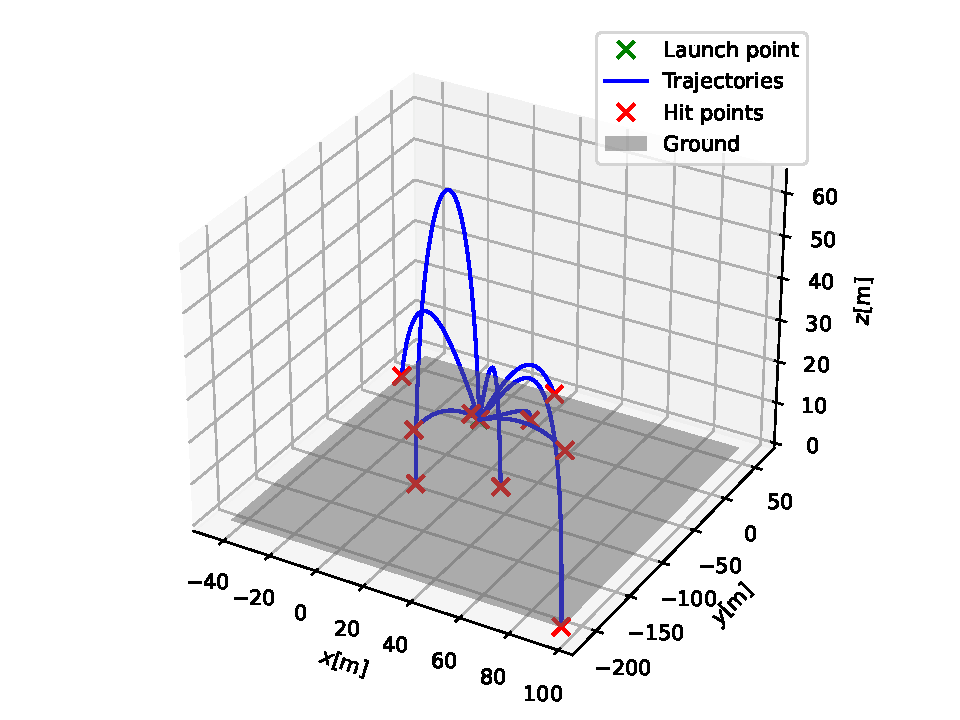
\includegraphics[width=\linewidth]{../figures/sample_trajectories_3d.pdf}
    \caption{Example 3D trajectories generated by the simulation. The curves illustrate the diversity of flight paths caused by different launch speeds, directions, drag strengths, wind vectors, and Magnus parameters.}
    \label{fig:sample_trajectories_3d}
\end{figure}

Overall, the simulation provides a controlled synthetic dataset with known physical parameters and tunable sources of trajectory variation.
This makes it possible to systematically study how different machine learning models behave when trained on full trajectories, engineered features, noisy observations, or cropped partial trajectories.


\section{Methods \label{sec:methods}}

This section describes the machine learning methods used to infer physical launch and environmental parameters from simulated projectile trajectories.
Two complementary model classes are considered: a multilayer perceptron (MLP) applied to manually engineered scalar trajectory descriptors, and gated recurrent unit (GRU) networks applied directly to time-resolved trajectory data.
The overall motivation is to compare a compact feature-based representation against a sequence-based representation that can, in principle, learn relevant temporal structure directly from the observed motion.

\subsection{Feature-Based Regression with a Multilayer Perceptron}

As a non-recurrent baseline, we use a multilayer perceptron that maps a fixed-dimensional vector of scalar trajectory features to the desired physical target parameters.
In the implementation, the MLP first flattens the input, then applies a sequence of fully connected linear layers with ReLU activations, followed by a final linear output layer.
For an input feature vector $\vb{x}\in\mathbb{R}^{d_{\mathrm{in}}}$, the model can be written schematically as
\begin{align*}
    \vb{h}_1 &= \sigma\left(W_1 \vb{x} + \vb{b}_1\right), \\
    \vb{h}_{\ell+1} &= \sigma\left(W_{\ell+1}\vb{h}_{\ell}+\vb{b}_{\ell+1}\right), \qquad \ell = 1,\dots,L-1, \\
    \hat{\vb{y}} &= W_{\mathrm{out}}\vb{h}_{L} + \vb{b}_{\mathrm{out}},
\end{align*}
where $\sigma$ denotes the ReLU\cite{nair2010rectified} activation function and $\hat{\vb{y}}$ is the predicted target vector.
The MLP experiments use scalar inputs with $24$ engineered features, and the output dimension is either $3$ for predicting the Cartesian initial velocity or $11$ for predicting the full set of selected launch and environmental parameters.

The scalar features are designed to summarize the most important geometric and kinematic properties of the trajectory.
They include the initial and final positions $(x_0,y_0,z_0)$ and $(x_T,y_T,z_T)$, the total flight time $T$, the displacement components $(\Delta x,\Delta y,\Delta z)$, the Euclidean start-to-end distance, the total arc length of the trajectory, the apex position $(x_{\mathrm{peak}},y_{\mathrm{peak}},z_{\mathrm{peak}})$, the time of the apex $t_{\mathrm{peak}}$, and finite-difference estimates of the initial and final velocity components and speeds.
These quantities provide physically interpretable information about range, curvature, maximum height, flight duration, and endpoint behavior.
For example, the initial finite-difference velocity estimate is computed from the first two sampled trajectory points, while the final velocity estimate is computed from the last two sampled points.
The total trajectory length is computed by summing the Euclidean distances between successive sampled positions.
The apex is identified as the point of maximal height $z$, which gives both the peak position and the corresponding time.

For some experiments, the desired target is not the spherical launch representation $(v_0,\theta,\phi)$, but the Cartesian initial velocity $(v_x,v_y,v_z)$.
This target is computed using
\begin{equation*}
    \pmqty{v_x\\v_y\\v_z} = v_0\pmqty{\sin\theta\cos\phi\\\sin\theta\sin\phi\\\cos\theta}
\end{equation*}
which is implemented as a preprocessing target transformation.
Using Cartesian velocity components avoids angular discontinuities in $\phi$ and gives a target representation that is often easier for regression models to learn.

\subsection{Sequence-Based Regression with Gated Recurrent Units}

The second model class is based on gated recurrent units, which are recurrent neural networks designed to process sequential data.
Instead of receiving a single engineered feature vector, the GRU receives a time series of trajectory observations such as
\begin{equation*}
    \vb{x}_1,\vb{x}_2,\dots,\vb{x}_T, \qquad \vb{x}_t = \begin{pmatrix}
        t_t & x_t & y_t & z_t
    \end{pmatrix}^{\top},
\end{equation*}
or an extended version that also contains velocity and acceleration estimates.
The GRU then returns a final hidden state, which is passed through a small feed-forward prediction head consisting of a linear layer, ReLU activation, dropout, and a final linear layer.
In the endpoint-augmented variants, a second prediction head is added to predict the two-dimensional hit point separately from the physical parameter vector.

A GRU updates its hidden state using gating mechanisms that control how much past information is retained and how much new information is incorporated.
For an input $\vb{x}_t$ and previous hidden state $\vb{h}_{t-1}$, the standard GRU equations are
\begin{align*}
    \vb{z}_t &= \sigma\left(W_z \vb{x}_t + U_z \vb{h}_{t-1} + \vb{b}_z\right), \\
    \vb{r}_t &= \sigma\left(W_r \vb{x}_t + U_r \vb{h}_{t-1} + \vb{b}_r\right), \\
    \tilde{\vb{h}}_t &= \tanh\left(W_h \vb{x}_t + U_h(\vb{r}_t \odot \vb{h}_{t-1}) + \vb{b}_h\right), \\
    \vb{h}_t &= (1-\vb{z}_t)\odot \vb{h}_{t-1} + \vb{z}_t \odot \tilde{\vb{h}}_t.
\end{align*}
Here, $\vb{z}_t$ is the update gate, $\vb{r}_t$ is the reset gate, $\tilde{\vb{h}}_t$ is the candidate hidden state, and $\odot$ denotes element-wise multiplication.\cite{cho2014gru}
The update gate allows the network to preserve information over many time steps, while the reset gate controls how strongly the previous hidden state contributes to the candidate state.
This makes GRUs suitable for time-series analysis because they learn a compressed representation of the trajectory history rather than treating each time point independently.
In this project, the final hidden state $\vb{h}_T$ is interpreted as a learned summary of the observed flight path and is used to predict the physical parameters.

The GRU models are particularly appropriate for this problem because projectile trajectories contain temporally ordered information.
Quantities such as curvature, deceleration, and asymmetry are not fully described by individual positions alone, but by their evolution over time.
A recurrent architecture can use early and late parts of the trajectory jointly, and it can also be evaluated on cropped sequences, where only a prefix of the trajectory is available.\cite{cho2014gru}
The training code supports random cropping of time-series batches by selecting only the first $k$ time points, where $k$ is sampled between fractions of the full sequence length.
This allows the model to learn from partial trajectories and is useful for studying how much of the flight path is needed to infer the underlying launch and environmental parameters.

\subsection{Data Preprocessing and Representation}

The raw simulator output consists of time arrays, three-dimensional positions, launch parameters, and metadata stored in immutable raw samples.
During preprocessing, each raw sample is converted into a processed representation containing trajectory channels $t,x,y,z$, scalar features, targets, and optionally metadata.
The dataset builder applies a configurable pipeline of transformations to each raw sample and then writes the selected features and targets into PyTorch tensors.
For time-series data, the resulting feature tensor has shape
\begin{equation*}
    (N, n_{\mathrm{features}}, n_{\mathrm{timepoints}}),
\end{equation*}
whereas scalar-feature data are stored as
\begin{equation*}
    (N, n_{\mathrm{features}}).
\end{equation*}
The target tensor has shape $(N,n_{\mathrm{targets}})$ in both cases.

A central preprocessing step for the GRU models is resampling.
Although the raw trajectories were generated with many time points, the GRU experiments use a reduced fixed-length representation with $100$ time points.
The resampling transform first chooses new time points between the minimum and maximum time of the trajectory and then interpolates the trajectory channels using a cubic spline.\cite{de1978practical}
The implemented sampling distributions include even, logarithmic, uniform, and Gaussian sampling over the normalized time interval.
In the main GRU training configurations, even resampling is used, so the trajectory is represented by uniformly spaced time samples.
This reduces computational cost while preserving a standardized input length for mini-batch training.

Additional time-series features are obtained by numerical differentiation.
Velocity channels are computed as
\begin{equation*}
    v_i(t) \approx \dv{r_i}{t}, \qquad i\in\{x,y,z\},
\end{equation*}
using numerical gradients of the position channels with respect to time.
Acceleration channels are then computed analogously from the velocity channels.
Some GRU configurations therefore use only $(t,x,y,z)$, while others use the extended feature set $(t,x,y,z,v_x,v_y,v_z,a_x,a_y,a_z)$.
The motivation for adding velocities and accelerations is that the forces in the physical simulation act through velocity-dependent drag and Magnus terms, so derivative information may make the underlying parameters easier to identify.
At the same time, numerical differentiation can amplify noise, so the benefit of these features must be evaluated empirically. \cite{chartrand2011numerical}

All models use standardization of features and targets. Standardization transforms each feature to have zero mean and unit variance, ensuring that all input features are on a comparable scale. This improves the stability and efficiency of gradient-based optimization, allowing neural networks to converge faster and preventing features with larger numerical values from disproportionately influencing the learning process.\cite{lecun2012efficient}
For scalar inputs, feature means and standard deviations are computed over the training samples, while for time-series inputs they are computed over both the sample and time dimensions for each feature channel.
Targets are standardized using the training-set mean and standard deviation for each output dimension.
The standardized quantities are therefore
\begin{equation*}
    \tilde{x} = \frac{x-\mu_x}{\sigma_x+\epsilon}, \qquad \tilde{y} = \frac{y-\mu_y}{\sigma_y+\epsilon},
\end{equation*}
with a small numerical constant $\epsilon=10^{-8}$ used for stability.
The same scaling factors are then applied to the corresponding test data, which avoids information leakage from the test set into the training process.
For later standalone evaluation runs, the saved feature and target scaling factors can be loaded and reused.


\section{Experimental Setup}
\label{sec:experimental_setup}

\subsection{Dataset Split and Preprocessing}

All experiments use the same repository of $N=200000$ simulated trajectories described in Section \ref{sec:data}. A pseudo-random permutation divides the data into $160000$ training trajectories and $40000$ test trajectories. The latter split is used to control the learning-rate scheduler, select the best checkpoint, and report the final metrics.

The scalar features and time-series channels are standardized as described in Section \ref{sec:methods}. Only statistics of the training split are used, and the same saved statistics are applied during all later evaluations. For the GRU models, each raw trajectory is represented by $100$ evenly spaced samples obtained by cubic-spline interpolation. The noise-free trajectory is used to construct all targets, including the impact point in the endpoint-augmented models.

\subsection{Model Configurations}

Table \ref{tab:model_configurations} summarizes the eight configurations. The two MLPs receive the $24$ engineered features introduced in Section \ref{sec:methods}. The first MLP predicts only the Cartesian initial velocity, whereas the second predicts all $11$ launch and environmental parameters.
The GRU prediction head maps the final hidden state through a $128$-unit linear layer, a ReLU activation, dropout with probability $0.1$, and a final linear output layer. Two-layer GRUs additionally use dropout $0.1$ between recurrent layers.
Configurations denoted by \enquote{derivatives} receive the ten channels
\begin{equation*}
    (t,x,y,z,v_x,v_y,v_z,a_x,a_y,a_z),
\end{equation*}
whereas the remaining GRUs receive only $(t,x,y,z)$.

\begin{table*}[htbp]
    \centering
    \small
    \resizebox{\textwidth}{!}{%
    \begin{tabular}{llllll}
        \hline
        ID & Model & Input & Architecture & Output & Crop augmentation \\
        \hline
        01 & MLP velocity & 24 scalar features & $64,32$ & $v_x,v_y,v_z$ & no \\
        02 & MLP all parameters & 24 scalar features & $128,64,32$ & 11 parameters & no \\
        03 & GRU positions & 4 channels & 1 layer, $h=128$ & 11 parameters & no \\
        04 & GRU derivatives & 10 channels & 2 layers, $h=128$ & 11 parameters & no \\
        05 & GRU cropped & 4 channels & 1 layer, $h=128$ & 11 parameters & $f\in[0.2,1.0]$ \\
        06 & GRU cropped derivatives & 10 channels & 2 layers, $h=128$ & 11 parameters & $f\in[0.2,1.0]$ \\
        07 & GRU cropped + endpoint & 4 channels & 1 layer, $h=128$ & 11 parameters + 2D endpoint & $f\in[0.2,1.0]$ \\
        08 & GRU cropped derivatives + endpoint & 10 channels & 2 layers, $h=128$ & 11 parameters + 2D endpoint & $f\in[0.2,1.0]$ \\
        \hline
    \end{tabular}}
    \caption{Model configurations used in the experiments. The symbol $f$ denotes the observed fraction of a trajectory.}
    \label{tab:model_configurations}
\end{table*}

During crop-augmented training, a single prefix length is sampled uniformly between $20$ and $100$ time points for each mini-batch, and the same length is used for every trajectory in that batch. For configurations 07 and 08, the test loss used during training is evaluated at $f=0.5$.
Their two heads minimize
\begin{equation}
    \mathcal{L}
    =
    \f{MSE}\left(\hat{\vb{\lambda}},\vb{\lambda}\right)
    + 0.5\,
    \f{MSE}\left(\hat{\vb{r}}_{\mathrm{hit}},\vb{r}_{\mathrm{hit}}\right),
    \label{eq:endpoint_loss}
\end{equation}
where both target blocks are standardized separately before the loss is computed.

\subsection{Optimization and Model Selection}

All models are optimized with Adam using a batch size of $256$, an initial learning rate of $10^{-3}$, and mean squared error in standardized target space.\cite{kingma2017adammethodstochasticoptimization}
A \texttt{ReduceLROnPlateau} scheduler multiplies the learning rate by $0.1$ after $10$ epochs without improvement, down to a minimum of $10^{-6}$. Early stopping is configured with a tolerance of $32$ non-improving epochs. The checkpoint with the lowest test loss is retained and used in every subsequent evaluation.\cite{bottou2018optimization}

The data permutation is reproducible because its seed is set explicitly. However, due to processing power constraints, only one trained instance of each configuration is available.The reported differences therefore describe these particular training runs. Uncertainty across initializations is not quantified.

The whole machine learning framework is implemented using PyTorch.\cite{paszke2019pytorch}
Additional numerical calculations are performed using the NumPy and SciPy libraries.\cite{harris2020array}\cite{virtanen2020scipy}
Visualizations and plots are realized in Matplotlib.\cite{hunter2007matplotlib}


\section{Evaluation}
\label{sec:evaluation}

\subsection{Regression Metrics}

Metrics are computed after undoing target standardization, separately for every physical output.
For target $j$, with residual $e_{ij}=\hat{y}_{ij}-y_{ij}$ on $n$ test samples, the principal metrics are
\begin{align}
    \operatorname{RMSE}_j
        &= \sqrt{\frac{1}{n}\sum_{i=1}^{n}e_{ij}^{\,2}}, \\
    \operatorname{MAE}_j
        &= \frac{1}{n}\sum_{i=1}^{n}\abs{e_{ij}}, \\
    R_j^2
        &= 1-\frac{\sum_i e_{ij}^{\,2}}
        {\sum_i\left(y_{ij}-\bar{y}_j\right)^2}.
\end{align}
RMSE retains the unit of the corresponding target and penalizes large errors more strongly than MAE, while $R^2$ is dimensionless. Median and maximum absolute error, explained variance, mean bias, residual standard deviation, Pearson correlation, MAPE, and sMAPE are also recorded. Percentage errors are not used as primary evidence because several Cartesian and spin-direction components can be close to zero, for which relative errors become unstable.\cite{chicco2021coefficient}

The supplied sweep plots flatten all output components before calculating an \enquote{overall RMSE}. Since the $11$ targets include velocities, dimensionless spin components, $\beta_D$ in $\si{\per\meter}$, and $\beta_M$ in $\si{\per\second}$, this aggregate is not a dimensionally meaningful physical error. Figures \ref{fig:cropping_performance} and \ref{fig:noise_performance} are therefore used only to visualize qualitative model trends. Quantitative comparisons are based on per-target metrics.

\subsection{Robustness Protocol}

The cropping sweep evaluates all six GRUs on deterministic trajectory prefixes
\begin{equation*}
    f\in\{0.1,0.2,\ldots,1.0\}.
\end{equation*}
For a sequence of length $T=100$, the model receives the first $\max(2,\lfloor fT\rfloor)$ samples. The sweep uses the same $40000$ test trajectories and targets at every fraction. It therefore isolates sensitivity to the amount of observed flight history.

For the noise sweep, independent zero-mean Gaussian perturbations are added to every resampled position coordinate and time point,
\begin{equation}
    \tilde{\vb{r}}_k
    =
    \vb{r}_k+\vb{\epsilon}_k,
    \qquad
    \vb{\epsilon}_k\sim\mathcal{N}\!\left(\vb{0},\sigma^2 I_3\right),
\end{equation}
with
\begin{equation*}
    \sigma\in
    \SIlist{0;0.01;0.02;0.05;0.10;0.20;0.50;1.00}{\meter}.
\end{equation*}
The noise is applied after resampling but before velocity and acceleration channels are computed and before saved clean-data standardization factors are applied. Thus, $\sigma$ is expressed in metres, and derivative-based models also receive derivatives of the noisy positions.\cite{chartrand2011numerical}
The physical trajectories themselves are not re-simulated: the preprocessing pipeline is rebuilt from the same raw repository, and the same split indices are reproduced.


\section{Results}
\label{sec:results}

\subsection{Training Behaviour}

The training and test loss curves decrease for all eight configurations, as illustrated schematically in Figure \ref{fig:loss_curves}. The curves labelled \enquote{test} in the generated plots correspond to the test model-selection split defined above.
The selected checkpoint occurs at epoch $953$ for the velocity-only MLP and at epoch $947$ for the all-parameter MLP. For the GRUs, the selected epochs are $413$, $159$, $343$, $251$, $399$, and $390$ for configurations 03--08, respectively.
Because the objectives contain different numbers and types of standardized outputs, especially for the endpoint models in Eq. \eqref{eq:endpoint_loss}, absolute loss values should not be compared directly across every configuration.

% \begin{figure}[htbp]
%     \centering
%     % \includegraphics[width=\linewidth]{figures/loss_curves_overview.pdf}
%     \fbox{\rule{0pt}{0.22\linewidth}\rule{0.92\linewidth}{0pt}}
%     \caption{Training and test loss as a function of epoch. The log--log representation makes both the rapid initial decrease and later convergence visible.}
%     \label{fig:loss_curves}
% \end{figure}

\begin{figure}[t]
  \centering

  \subfloat[\label{fig:loss_curve_02}]{
    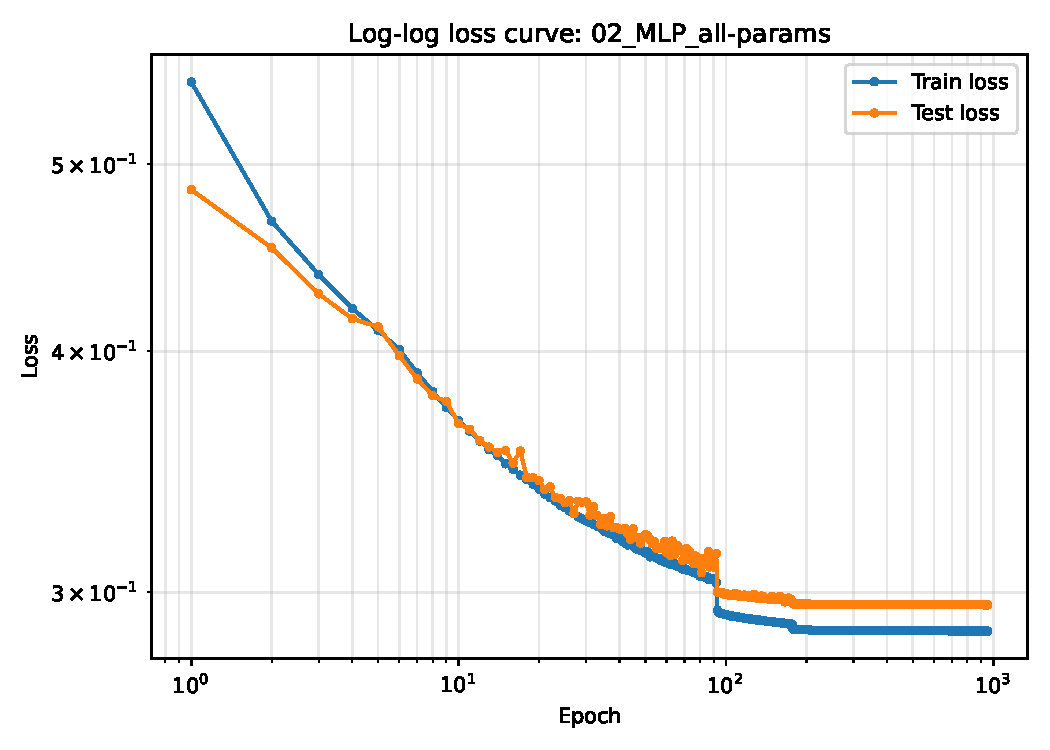
\includegraphics[width=\linewidth]{../figures/02_MLP_all-params_loss_curve_loglog}
  }

  \vspace{0.5em}

  \subfloat[\label{fig:loss_curve_05}]{
    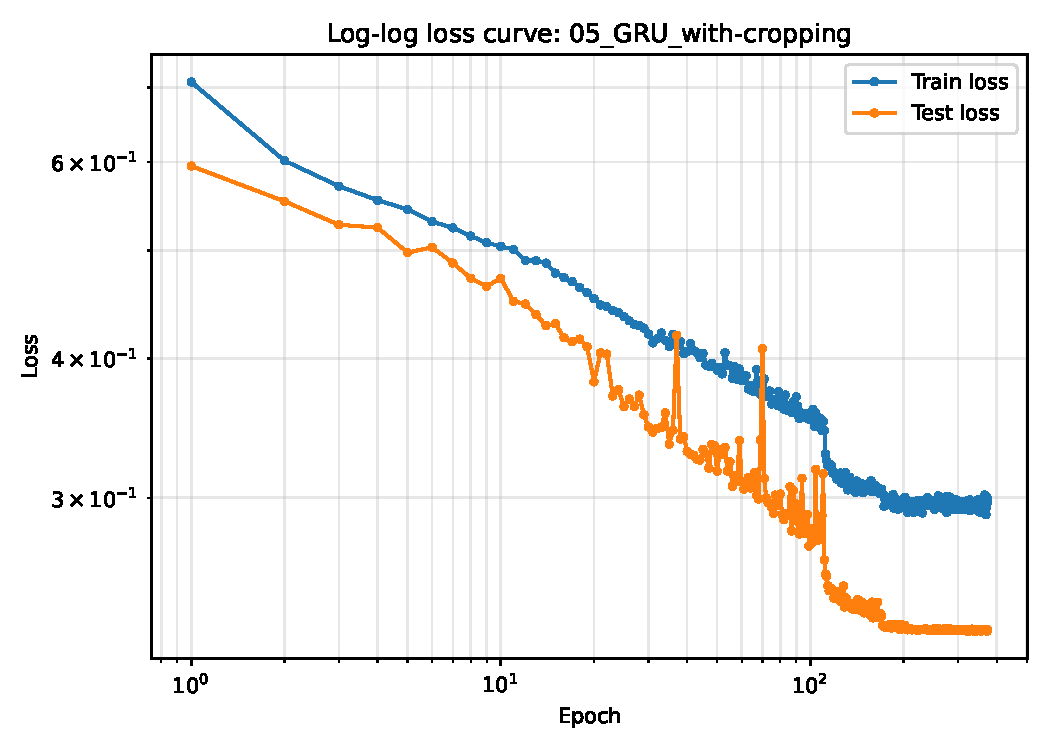
\includegraphics[width=\linewidth]{../figures/05_GRU_with-cropping_loss_curve_loglog}
  }

  \caption{Training and test loss as a function of epoch. The log-log representation makes both the rapid initial decrease and later convergence visible. Further loss curves can be found in the appendix (see Sec. \ref{sec:appendix}).}
  \label{fig:loss_curves}
\end{figure}

\subsection{Performance on Complete, Noise-Free Trajectories}

The velocity-only MLP achieves RMSE values of
$\SI{0.00640}{\meter\per\second}$,
$\SI{0.00677}{\meter\per\second}$, and
$\SI{0.00304}{\meter\per\second}$
for $v_x$, $v_y$, and $v_z$, respectively. This near-exact reconstruction is expected because its engineered inputs include a finite-difference estimate of the initial velocity. It should therefore be interpreted as a task-specific feature-engineering baseline rather than as evidence that the remaining physical parameters are equally identifiable.

Table \ref{tab:clean_results} compares representative outputs for the all-parameter models.
The MLP remains competitive for launch velocity, but the GRUs recover wind, spin direction, drag, and Magnus strength more accurately. Adding velocity and acceleration channels to the full-trajectory GRU reduces the RMSE of $u_x$ from
$\SI{2.67}{\meter\per\second}$ to $\SI{1.36}{\meter\per\second}$, of $\beta_D$ from
$\SI{0.00300}{\per\meter}$ to $\SI{0.00127}{\per\meter}$, and of $\beta_M$ from
$\SI{0.0378}{\per\second}$ to $\SI{0.0190}{\per\second}$.
The corresponding $R^2$ values increase from $0.899$ to $0.974$, from $0.920$ to $0.986$, and from $0.810$ to $0.952$, respectively.

\begin{table}[htbp]
    \centering
    \small
    \resizebox{\linewidth}{!}{%
    \begin{tabular}{lllll}
        \hline
        Target & MLP all & GRU positions & GRU derivatives & GRU cropped derivatives \\
        \hline
        $v_x\,[\si{\meter\per\second}]$
            & $1.016\;(0.998)$ & $1.793\;(0.995)$ & $1.027\;(0.998)$ & $1.223\;(0.998)$ \\
        $u_x\,[\si{\meter\per\second}]$
            & $3.857\;(0.789)$ & $2.667\;(0.899)$ & $1.359\;(0.974)$ & $1.413\;(0.972)$ \\
        $\omega_x$
            & $0.413\;(0.488)$ & $0.247\;(0.817)$ & $0.129\;(0.950)$ & $0.133\;(0.947)$ \\
        $\beta_D\,[\si{\per\meter}]$
            & $0.00445\;(0.825)$ & $0.00300\;(0.920)$ & $0.00127\;(0.986)$ & $0.00121\;(0.987)$ \\
        $\beta_M\,[\si{\per\second}]$
            & $0.0664\;(0.413)$ & $0.0378\;(0.810)$ & $0.0190\;(0.952)$ & $0.0191\;(0.952)$ \\
        \hline
    \end{tabular}}
    \caption{Per-target test performance on complete, noise-free trajectories. Each entry reports RMSE followed by $R^2$ in parentheses. Model names correspond to configurations 02, 03, 04, and 06 in Table~\ref{tab:model_configurations}.}
    \label{tab:clean_results}
\end{table}

Random-crop augmentation slightly sacrifices complete-trajectory accuracy for some outputs, but configuration 06 remains close to configuration 04. The endpoint-augmented derivative model likewise gives comparable parameter errors, for example $\operatorname{RMSE}(\beta_M)=\SI{0.0184}{\per\second}$.
Its endpoint MAEs are $\SI{1.22}{\meter}$ in $x$ and $\SI{1.17}{\meter}$ in $y$, while the corresponding RMSEs are $\SI{4.65}{\meter}$ and $\SI{3.35}{\meter}$. The gap between MAE and RMSE indicates that a minority of comparatively large endpoint errors remains. The auxiliary endpoint objective does not yield a consistent improvement of the $11$ physical-parameter predictions over configuration 06.

\subsection{Dependence on the Observed Trajectory Fraction}

Figure \ref{fig:cropping_performance} shows that GRUs trained only on complete trajectories deteriorate strongly when only an early prefix is available. Crop augmentation substantially reduces this distribution shift. For configuration 06 at $f=0.5$, the RMSEs are $\SI{1.08}{\meter\per\second}$ for $v_x$, $\SI{1.64}{\meter\per\second}$ for $u_x$, $0.150$ for $\omega_x$, $\SI{0.00136}{\per\meter}$ for $\beta_D$, and $\SI{0.0223}{\per\second}$ for $\beta_M$.
These values are close to the corresponding full-trajectory errors in Table \ref{tab:clean_results}. Even at $f=0.1$, configuration 06 yields $\operatorname{RMSE}(v_x)=\SI{2.16}{\meter\per\second}$, compared with $\SI{6.62}{\meter\per\second}$ for the derivative GRU trained only on complete trajectories. The remaining deterioration of wind, spin, and aerodynamic parameters at very small $f$ is physically plausible because these quantities influence curvature and deceleration over time, so their effects are only weakly expressed at the beginning of a flight.

\begin{figure}[htbp]
    \centering
    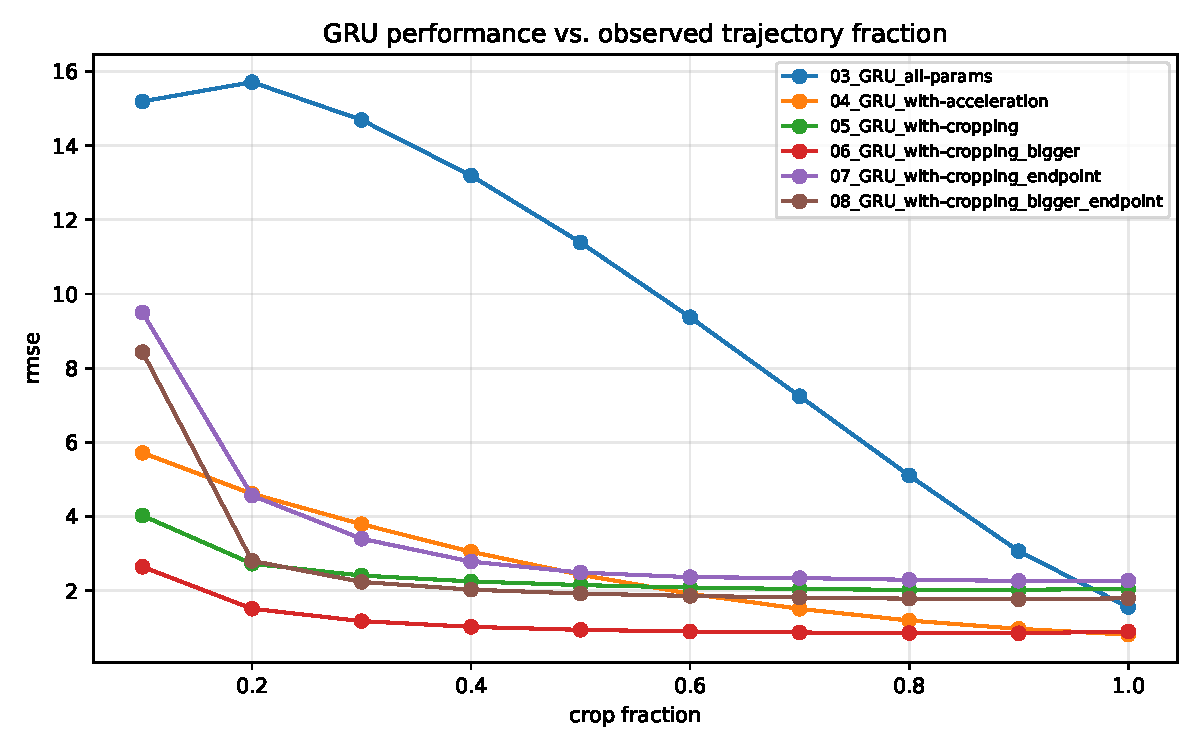
\includegraphics[width=0.92\linewidth]{../figures/gru_performance_vs_cropping.pdf}
    \caption{Diagnostic aggregate RMSE of the GRU configurations as a function of the observed trajectory fraction. Since the aggregate mixes outputs with different physical units, per-target values are used for quantitative interpretation.}
    \label{fig:cropping_performance}
\end{figure}

\subsection{Robustness to Gaussian Position Noise}

All GRUs are sensitive to measurement noise, and the degradation is already pronounced at $\sigma=\SI{0.01}{\meter}$, as shown in Figure \ref{fig:noise_performance}. For the derivative GRU without crop augmentation, the RMSE of $v_x$ increases from $\SI{1.03}{\meter\per\second}$ to $\SI{21.0}{\meter\per\second}$, while the RMSE of $u_x$ increases from $\SI{1.36}{\meter\per\second}$ to $\SI{9.50}{\meter\per\second}$. Over the same change, the $\beta_D$ error increases from $\SI{0.00127}{\per\meter}$ to $\SI{0.0120}{\per\meter}$. This behaviour is consistent with the fact that velocity and especially acceleration are obtained by differentiating already perturbed positions.

No single configuration dominates for every noisy target. At $\sigma=\SI{0.01}{\meter}$, the position-only endpoint model has a lower $v_x$ RMSE of $\SI{6.94}{\meter\per\second}$, but its $u_x$ RMSE is $\SI{20.3}{\meter\per\second}$, compared with $\SI{9.50}{\meter\per\second}$ for the derivative GRU. The results therefore reveal a trade-off between clean-data accuracy and target-dependent robustness. They also show that crop augmentation alone is not a substitute for noise augmentation: none of the training configurations adds Gaussian observation noise. A natural extension is to train with noise levels representative of the intended measurement system \cite{bishop1995training}, or to estimate derivatives using a smoothing or regularized procedure \cite{chartrand2011numerical}.

\begin{figure}[htbp]
    \centering
    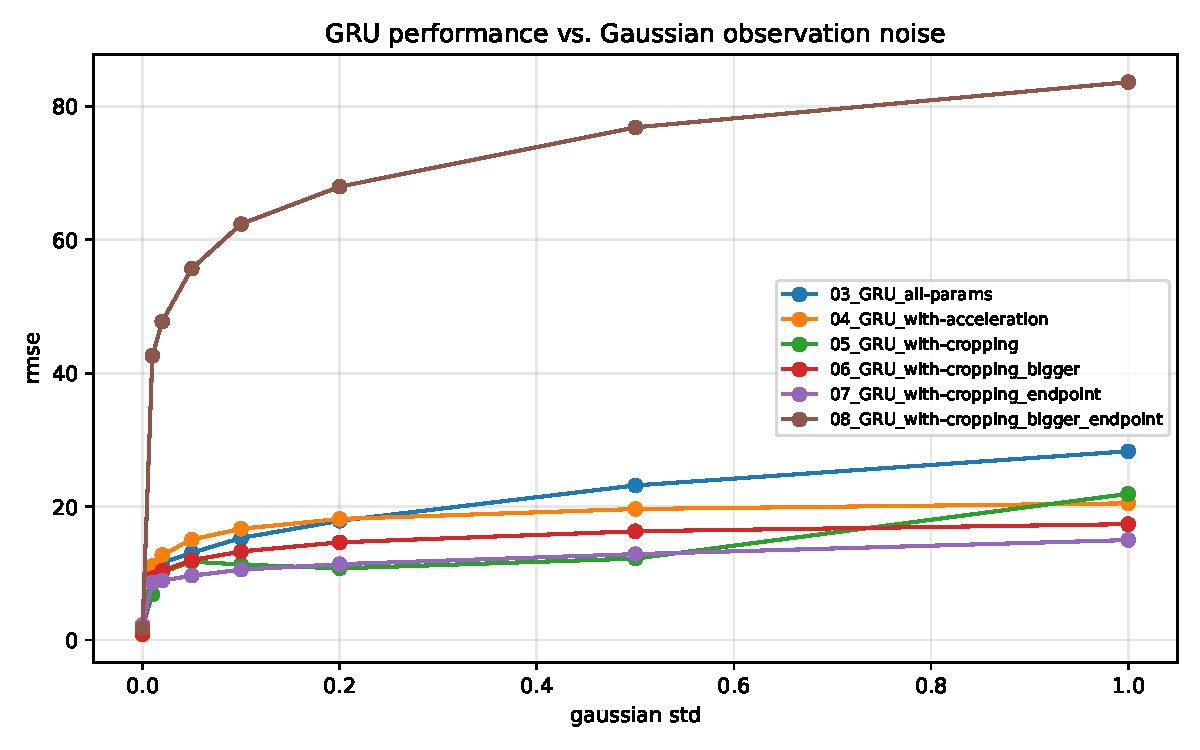
\includegraphics[width=0.92\linewidth]{../figures/gru_performance_vs_gaussian_noise.pdf}
    \caption{Diagnostic aggregate RMSE of the GRU configurations under independent Gaussian position noise. Noise is added before derivative features are computed. The aggregate curve is used qualitatively because it combines targets with different units.}
    \label{fig:noise_performance}
\end{figure}

Overall, engineered velocity features solve the restricted initial-velocity task extremely accurately, whereas sequence models are more effective for the joint inverse problem. For complete, clean trajectories, explicitly supplied derivatives provide the strongest overall parameter recovery. For partial trajectories, random-crop training is essential and retains useful accuracy down to substantially shorter prefixes. In contrast, the noise experiment exposes a major limitation of the present preprocessing pipeline: numerical derivatives improve clean-data accuracy but amplify positional noise.


\section{Conclusion}
\label{sec:conclusion}

This project compared feature-based MLPs and sequence-based GRUs for inferring physical parameters from simulated three-dimensional projectile trajectories. The restricted initial-velocity task was solved extremely accurately by an MLP using engineered features, with test RMSEs of $\SI{0.00640}{\meter\per\second}$, $\SI{0.00677}{\meter\per\second}$, and $\SI{0.00304}{\meter\per\second}$ for $v_x$, $v_y$, and $v_z$, respectively.
This result is primarily attributable to the inclusion of a finite-difference estimate of the initial velocity and therefore demonstrates the value of task-specific feature engineering. For the more demanding joint prediction of $11$ launch and environmental parameters, the GRU models generally outperformed the all-parameter MLP, particularly for wind, spin direction, drag, and Magnus strength.

On complete, noise-free trajectories, explicitly providing velocity and acceleration channels produced the most accurate overall parameter recovery. For example, relative to the position-only full-trajectory GRU, the derivative GRU reduced the test RMSE of $u_x$ from $\SI{2.67}{\meter\per\second}$ to $\SI{1.36}{\meter\per\second}$ and that of $\beta_D$ from $\SI{0.00300}{\per\meter}$ to $\SI{0.00127}{\per\meter}$.
Random-crop augmentation was essential when only a prefix of the flight was available. The crop-trained derivative model retained useful performance at short observation fractions and, at $f=0.1$, reduced the $v_x$ RMSE from $\SI{6.62}{\meter\per\second}$ for the model trained only on complete trajectories to $\SI{2.16}{\meter\per\second}$. The auxiliary impact-point objective did not consistently improve recovery of the physical parameters.

The Gaussian-noise experiments exposed the main weakness of the present approach. Although numerical derivatives are highly informative for clean inputs, differentiating perturbed positions amplifies measurement noise. For the derivative GRU, adding only $\sigma=\SI{0.01}{\meter}$ of positional noise increased the $v_x$ RMSE from $\SI{1.03}{\meter\per\second}$ to $\SI{21.0}{\meter\per\second}$. Crop augmentation did not prevent this degradation because none of the models was trained with noisy observations. Future work should therefore include noise augmentation matched to the measurement process and investigate smoothing, regularized differentiation, or architectures that infer kinematic information directly from positions.\cite{chartrand2011numerical}

The conclusions are limited to the simulated parameter ranges and physical assumptions used here. In addition, the same test split was used for checkpoint selection and final evaluation, only one training run was available for each configuration, and no independent simulated or experimental test set was used. Repeated training with controlled random seeds, a separate final test set, and validation on real trajectory measurements would be required for stronger claims about generalization and practical applicability. Within these limitations, the experiments show that GRUs can recover several latent physical parameters from trajectory data, provided that the training distribution reflects the expected degree of trajectory incompleteness and measurement noise.



\bibliography{references}% Produces the bibliography via BibTeX.

\section*{Appendix \label{sec:appendix}}
\clearpage
\begin{figure*}[h]
  \centering
  \subfloat[\label{fig:panel-a}]{
    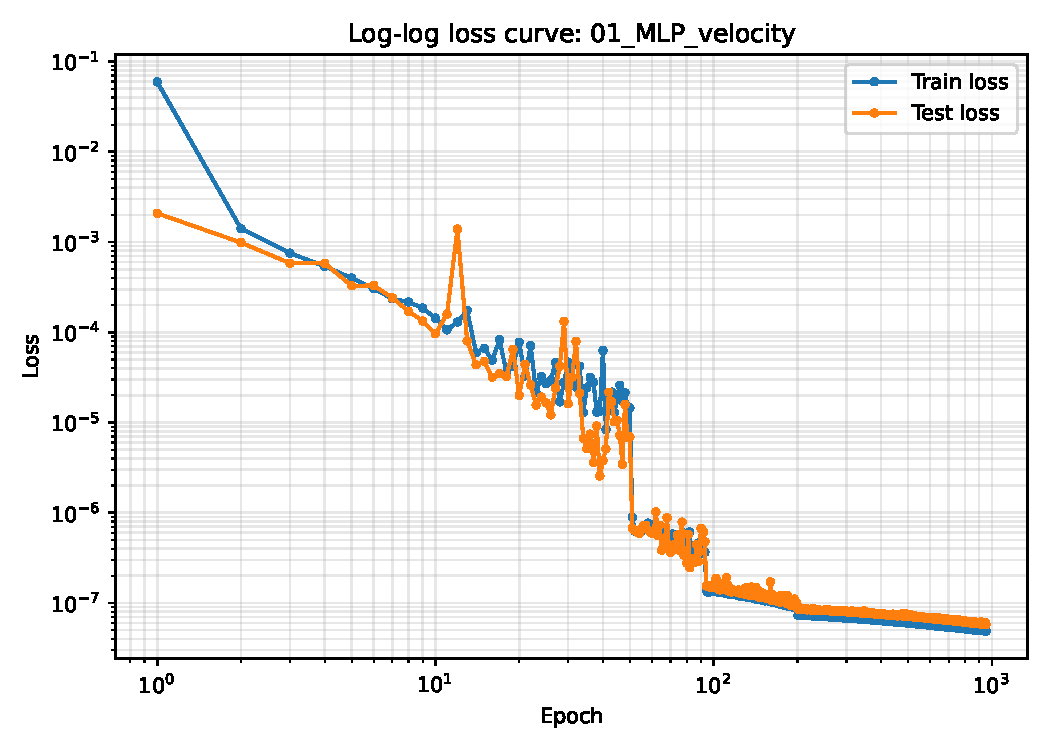
\includegraphics[width=0.48\textwidth]{../figures/appendix/01_MLP_velocity_loss_curve_loglog}
  }
  \hfill
  \subfloat[\label{fig:panel-b}]{
    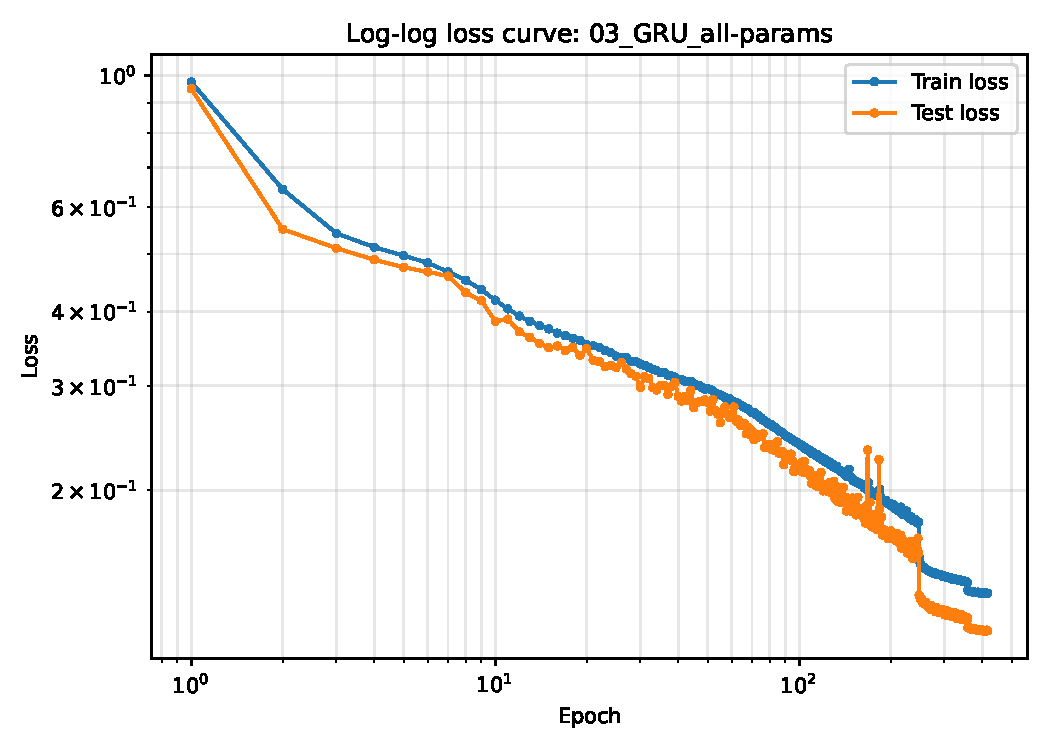
\includegraphics[width=0.48\textwidth]{../figures/appendix/03_GRU_all-params_loss_curve_loglog}
  }

  \par\vspace{0.8em}

  % Row 2
  \subfloat[\label{fig:panel-c}]{
    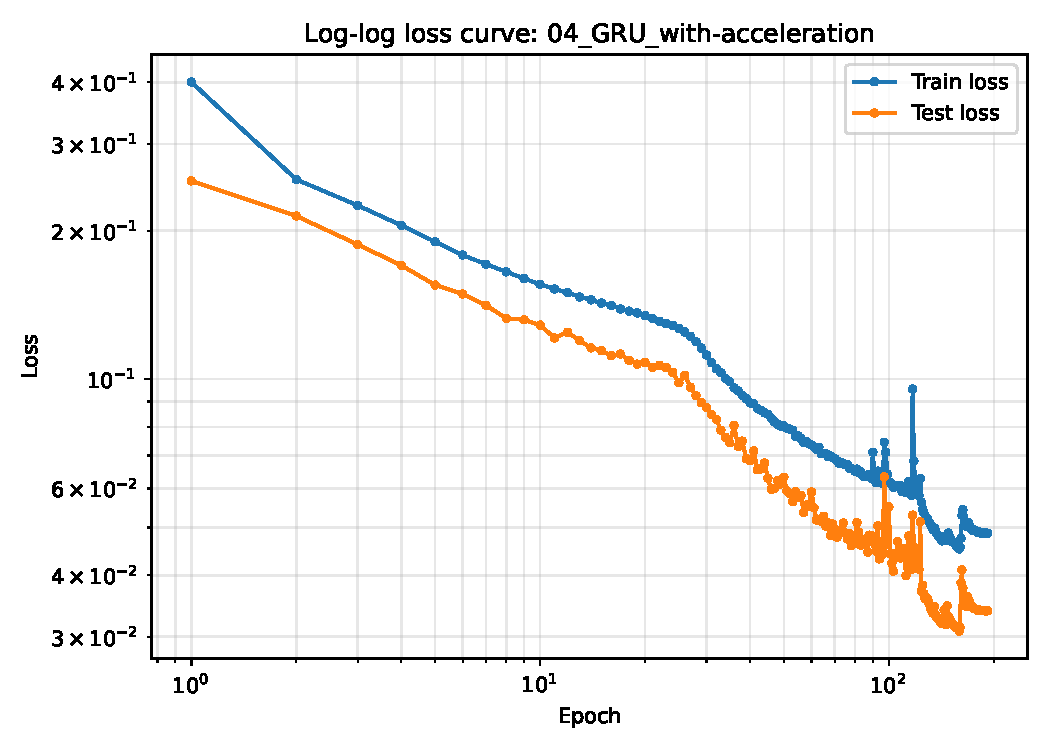
\includegraphics[width=0.48\textwidth]{../figures/appendix/04_GRU_with-acceleration_loss_curve_loglog}
  }
  \hfill
  \subfloat[\label{fig:panel-d}]{
    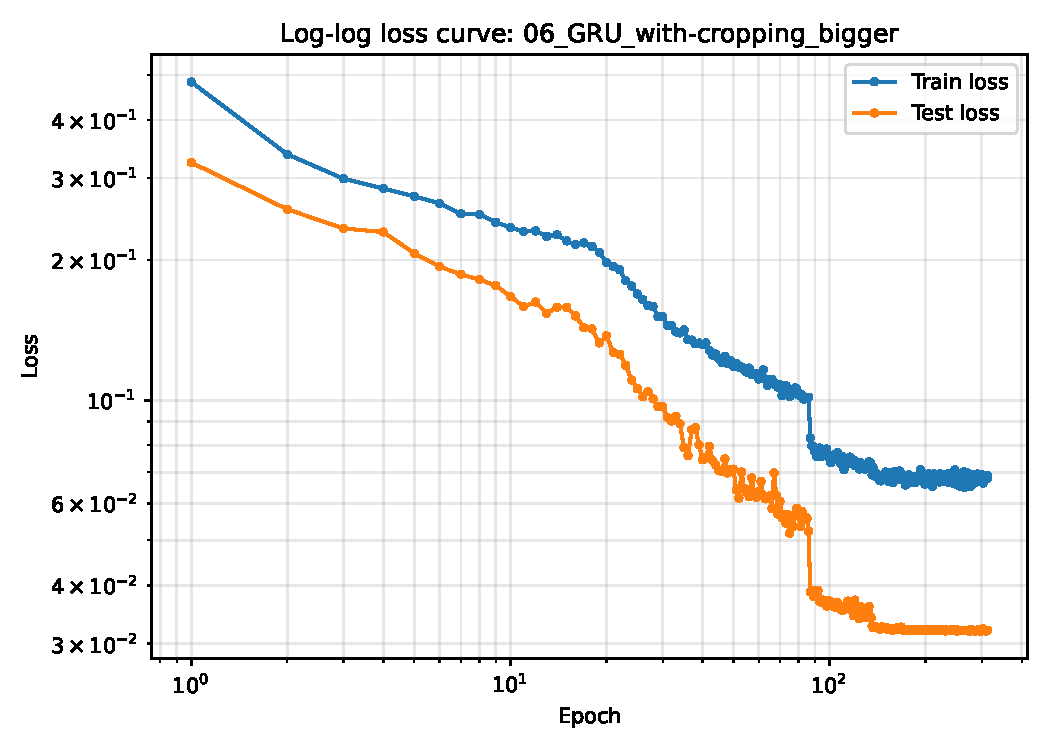
\includegraphics[width=0.48\textwidth]{../figures/appendix/06_GRU_with-cropping_bigger_loss_curve_loglog}
  }

  \par\vspace{0.8em}

  % Row 3
  \subfloat[\label{fig:panel-e}]{
    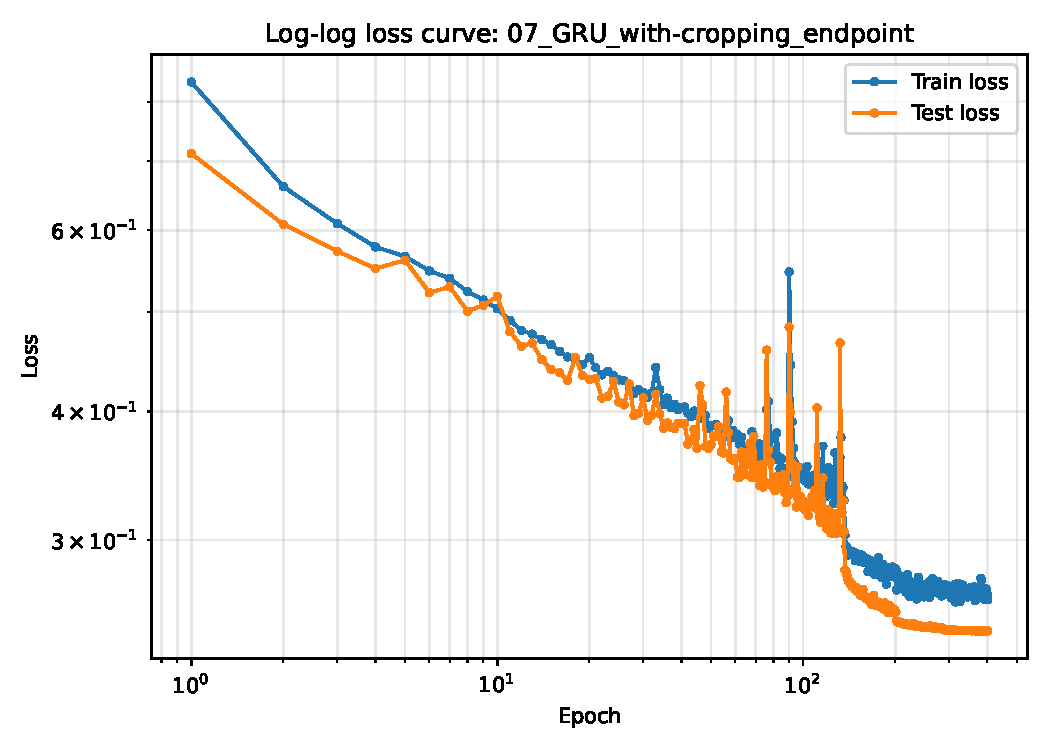
\includegraphics[width=0.48\textwidth]{../figures/appendix/07_GRU_with-cropping_endpoint_loss_curve_loglog}
  }
  \hfill
  \subfloat[\label{fig:panel-f}]{
    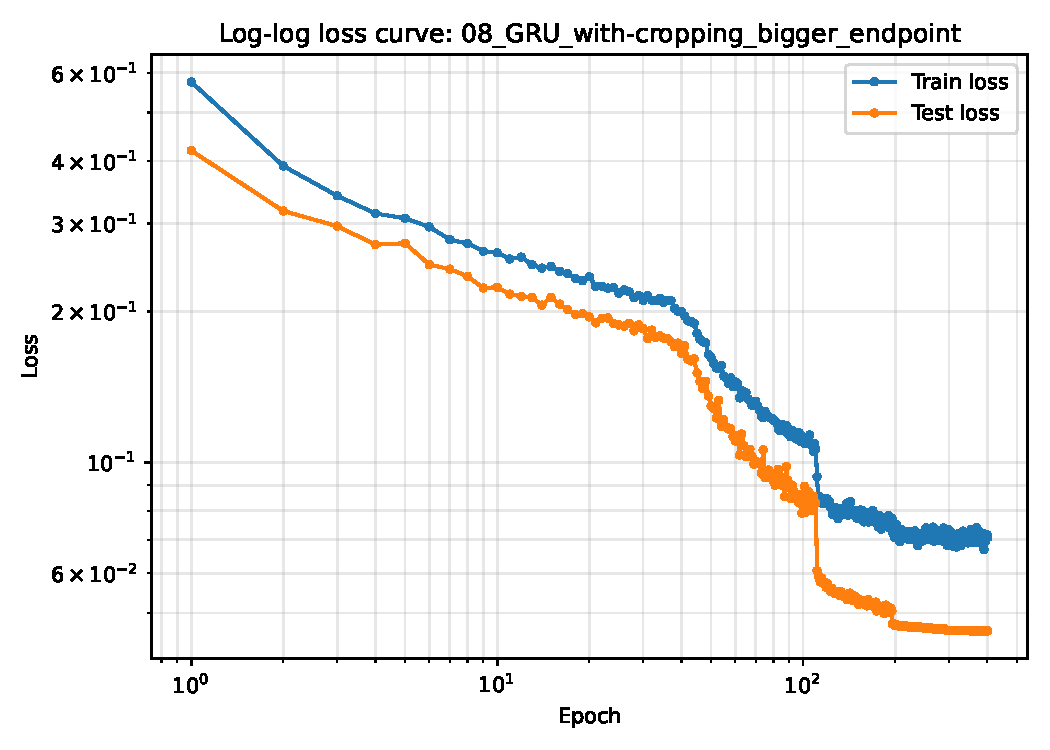
\includegraphics[width=0.48\textwidth]{../figures/appendix/08_GRU_with-cropping_bigger_endpoint_loss_curve_loglog}
  }

  \caption{Additional training run loss curves.}
  \label{fig:additional_loss_curves}
\end{figure*}



\end{document}
